\chapter{State of the Art}
\label{cha:StateOfTheArt}

Comparison of rigid and non-rigid\cite{survey}

\section{General pose capture workflow}
\label{PoseCapture}
Generally, there are two major steps to capture the pose of an object. First, the object has to be digitalized, which is achieved by a 3D scanning and reconstruction approach. The data might be in form of a point cloud or voxels depending on the reconstruction method (see section \ref{sec:reconstruction}). The second major step includes the analysis of the data to recognize body parts and subsequently joints and if required the skeleton. Depending on the chosen approach, which is usually a segmentation step (see section \ref{sec:segmentation}), there might be a subdivision into sub steps.
%
%TODO: new image with puppet! --> picture, point cloud, skeleton
%
\begin{figure}
	\centering
	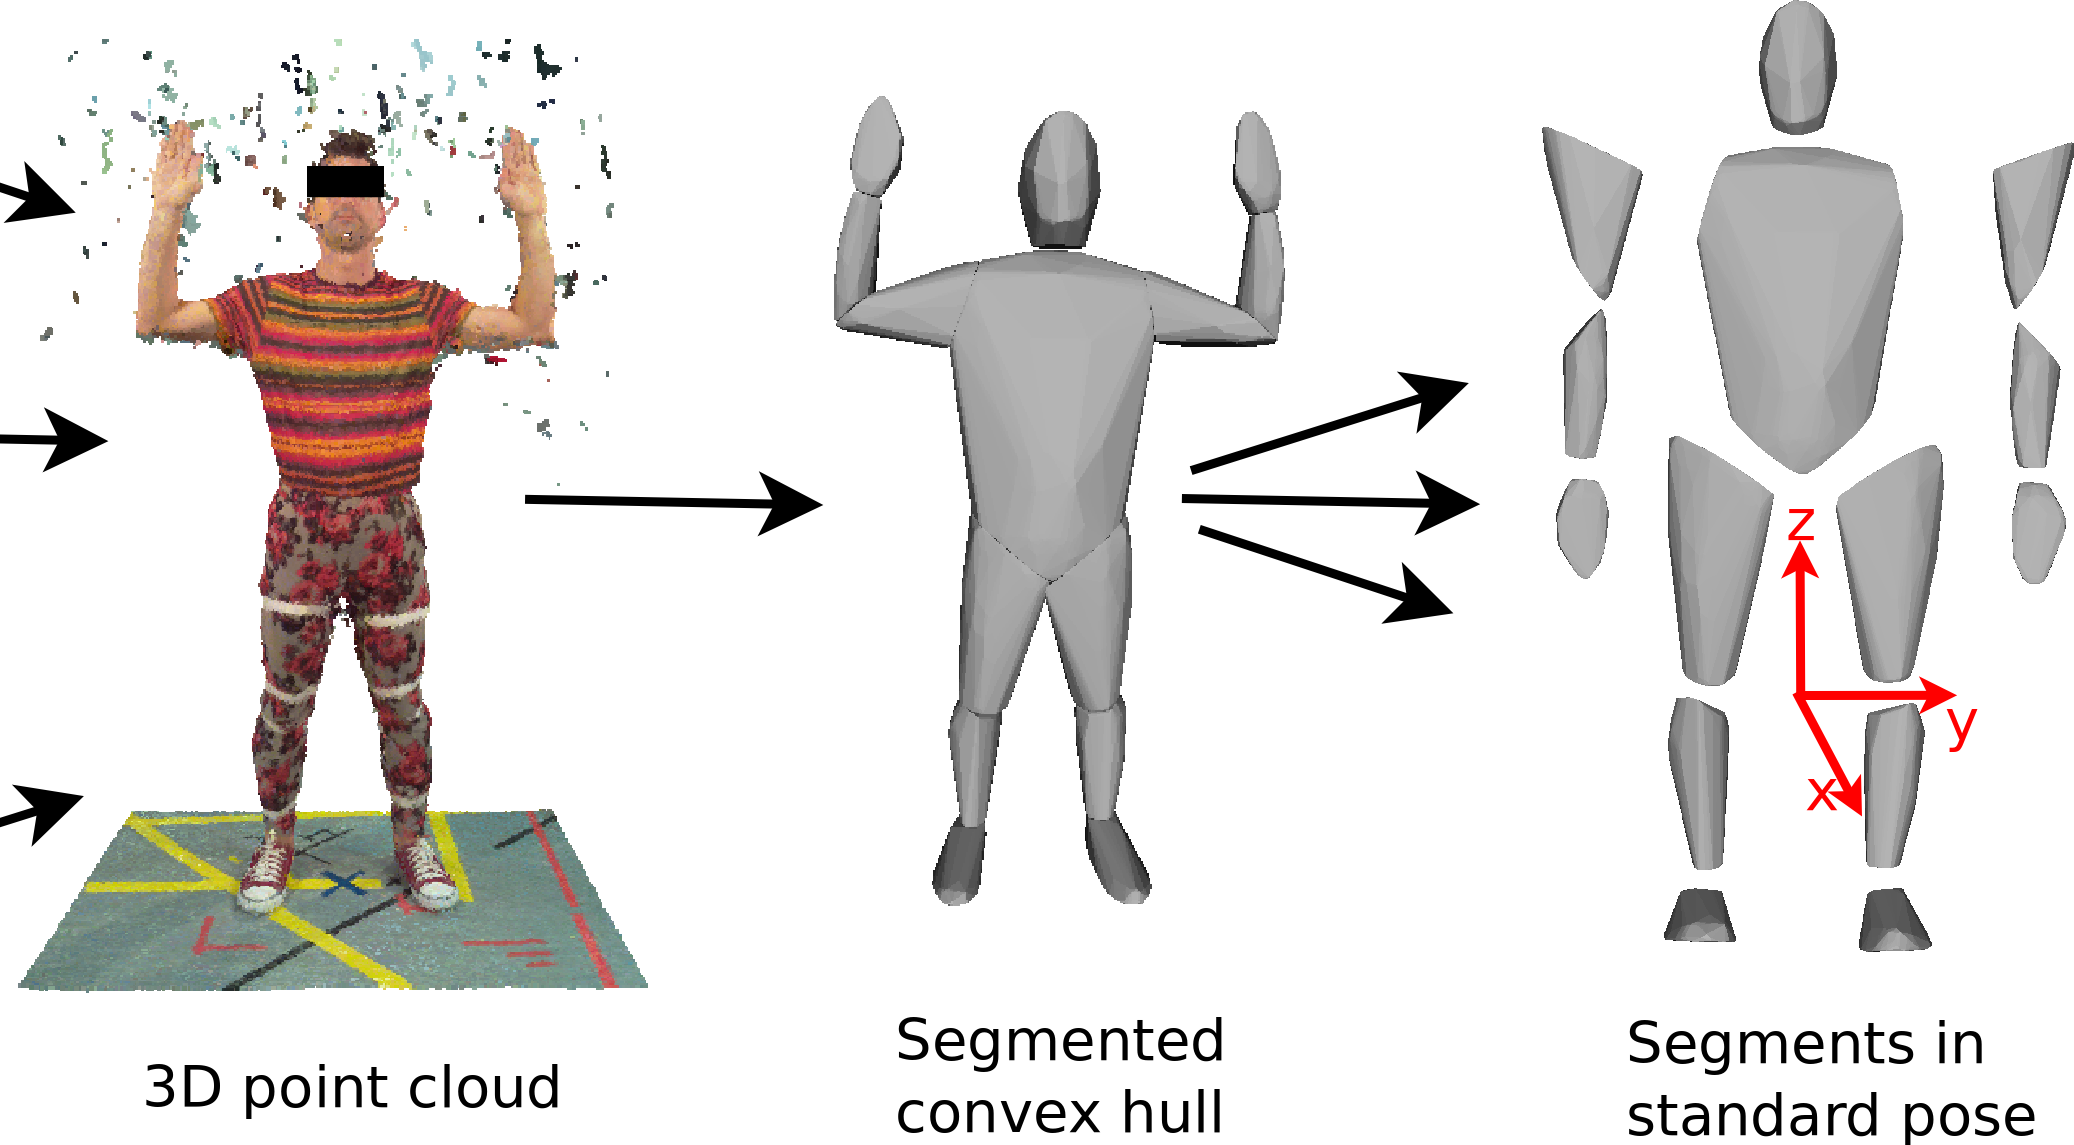
\includegraphics[width=0.7\linewidth]{reconstructionWorkflow}
	\caption{General approach to estimate the pose of a real object, including 3D scanning and reconstruction, 3D segmentation to get the joints and subsequently skeleton extraction}
	\label{fig:posecapture}
\end{figure}
%
\subsection{3D Scanning/Reconstruction}
\label{sec:reconstruction}
%
% ToDo: explain in detail
%
Scanning means collecting a real shape as 3D data. Reconstruction means the approach to convert the raw data to a mesh or process the input data.

Voxelization, Shape from Shilouette, Shape from Shading, Depth camera, stereo camera
%
%TODO: add all references (shape fitting, ...)
%
\subsection{3D Segmentation}
\label{sec:segmentation}
%
% ToDo: explain methods in detail
% 1) markers/sensors/exoskeleton
% 2) markerless methods
%
How it is done: markers, sensors, shape fitting (already known)
Cite all papers (Voxelization, ....). There are previous approaches with markers and sensors which will not be treated in this work in detail, as markerless options are taken as focus.

\section{Supervised methods}
Many already existing methods don't require markers and sensors but already assume or know the hierarchical structure or the body parts of the object to be captured (see \cite{multiLayerSkeleton}, \cite{baker2005shape}, \cite{de2008hierarchical} and \cite{michoud2007real}).

\section{Unsupervised methods}
Although the approaches mentioned in section \ref{sec:currentApproaches} work quite well depending on the application, improvements can be made that are more independent from user inputs. For example the computation of features, ... which leads us to the non-rigid registration \ref{nonrigidregistration}.

\subsection{Non-rigid registration}
\label{nonrigidregistration}

Generally, registration means the alignment of rigid point clouds (see figure \ref{fig:registration}). A well-known approach to achieve this, is the iterative closest point (ICP) \cite{ICP}, which requires the input point clouds to be aligned quite similar to avoid a local optimum. After registration, a matching error $e$ is achieved, which states the total euclidean distance between the associated points of the registered point clouds. In case of two non-rigid objects (e.g. a human in different poses which is composed of rigid parts) the ICP won't lead to a satisfying registration as associated parts are transformed differently. In order to register a non-rigid object, a segmentation into its rigid parts is required.

\subsection{Challenges}
\label{Challenges}
There are many challenges regarding the non-rigid registration of point clouds in 2D, as well as in 3D. First off, the input data can be noisy by means of points not belonging to the object. Furthermore, the approach is computationally expensive and time-consuming, as the corresponding body parts of two meshes need to be detected iteratively. Additionally, the inevitable difficulty of finding the global optimum, related to ambiguous body parts, has to be overcome.

\subsection{Related work}
\label{sec:RelatedWork}

By focusing on approaches computing the segmentation of articulated objects from 3D data, many different ones could be detected. They face similar challenges (see subsection \ref{Challenges}) but solve them in different ways
%%
\subsection{Correlated Correspondence}

A main approach for non-rigid registration is proposed by Anguelov \cite{Anguelov04} applying the correlated correspondence algorithm \cite{CorrelatedCorrespondance}. The algorithm takes a \textit{template} Mesh $D_0$ and other Meshes $D_1,\ldots,D_n$ in different configurations as input. The algorithm then performs a probabilistic framework and Expectation-Maximization (EM) to iterate between finding a decomposition of the \textit{template} into rigid parts and detecting them in the other meshes. Furthermore, a random clustering is applied to facilitate the detection of associated rigid parts.
%%
%TODO: images?
%%
A different approach proposes the recursive detection of body parts by the LRP -- ``largest rigid part'' algorithm \cite {guo2016correspondence}. 
%%
\subsection{LRP}
The LRP algorithm discovers the articulated parts of two objects in different configurations by initially detecting the largest rigid part. This would be the biggest point cluster by applying a single rigid transformation. To reach that, sparse correspondences in combination with RANSAC are implemented. From there, the linking parts are recursively detected by growing clusters from the LRP and reapplying the algorithm. 
%%
%TODO: images?
%%
Another approach is achieved by Symmetrization \cite{Mitra07}, by detecting and aligning the body parts’ symmetry axes of an object(see figure \ref{fig:Symmetrization}). Based on Anguelov \cite{Anguelov04} and Mitra \cite{Mitra07}, Chang et al developed a closely related approach \cite{chang08articulated} \cite{chang09range}.
%%
%TODO: images?
%%

%TODO: Add other references
\subsection{Possible improvements}

%TODO: What are the main deficits of the algorithms?

The proposed approaches achieve convincing results concerning the accuracy of the segmentation and the detection of rigid parts. However, they are all computationally expensive and require a considerable number of computation steps to iteratively detect rigid parts in two associated objects. This reflects on the run time of the algorithm which offers therefore great potential for improvements.

Taking the existing methods as reference (see chapter \ref{cha:RelatedWork}) a new segmentation approach is developed. Thereby, the main focus is to reduce the computation steps of the correlated correspondence algorithm \cite{CorrelatedCorrespondance} as well as the LRP algorithm \cite {guo2016correspondence}. To fully focus on the segmentation into its rigid part, the 3D reconstruction of the articulated object is assumed to be available.